%\documentclass[11pt]{article}
\documentclass[preprintnumbers,prd,superscriptaddress,notitlepage,nofootinbib] {revtex4-1}

\usepackage{geometry, amsmath, amsthm, latexsym, amssymb, graphicx,wasysym}
\usepackage[dvipsnames]{xcolor}
\geometry{margin=1in, headsep=0.25in}
%\usepackage[usenames, dvipsnames]{color}

% define units, short-names...

\newcommand{\frachalf}{\frac{1}{2}}
\newcommand{\dzbar}{\delta_{\bar{z}}}
\newcommand{\fNL}{f_{\rm NL}}
\newcommand{\kNL}{k_{\rm NL}}
\newcommand{\FoM}{{\rm FoM}}
\newcommand{\cm}{\ \text{cm}}
\newcommand{\pc}{\ \text{pc}}
\newcommand{\Mpc}{\ \text{Mpc}}
\newcommand{\Gpc}{\ \text{Gpc}}
\newcommand{\kpc}{\ \text{kpc}}
\newcommand{\Gyr}{\ \text{Gyr}}
\newcommand{\hkpc}{\ h^{-1}\text{kpc}}
\newcommand{\hMpc}{\ h^{-1}\text{Mpc}}
\newcommand{\hMpcc}{\ h^{-3}\text{Mpc}^3}
\newcommand{\hGpc}{\ h^{-1}\text{Gpc}}
\newcommand{\hGpcc}{\ h^{-3}\text{Gpc}^3}
\newcommand{\ihMpc}{\ h\text{Mpc}^{-1}}
\newcommand{\iMpc}{\ \text{Mpc}^{-1}}
\newcommand{\Ms}{\ M_\odot}
\newcommand{\hMs}{\ h^{-1} M_\odot}
\newcommand{\eh}[1]{\exp{\left[#1\right]}}
\newcommand{\tim}[1]{\times 10^{#1}}%times 10 
\newcommand{\unit}[1]{\ \text{#1}}
\newcommand{\tb}[1]{\textcolor{blue}{#1}}
\newcommand{\tr}[1]{\textcolor{red}{#1}}
\newcommand{\tsc}[1]{#1}
\newcommand{\derd}{\,\mathrm{d}} % upright d for derivatives and integrals
\newcommand{\ddir}{\delta^\text{(D)}}
\newcommand{\dkron}{\delta^\text{(K)}}
\newcommand{\be}{\begin{equation}}
\newcommand{\ee}{\end{equation}}
\newcommand{\la}{\left\langle}
\newcommand{\ra}{\right\rangle}
\newcommand{\derivd}{\text{d}}
\renewcommand{\vec}{\bm}
\newcommand{\FT}[1]{{\rm FT}\left[#1\right]}
\newcommand{\twopicub}{\left(2\pi\right)^3}
\newcommand{\intvkop}{\int\frac{\derivd^3k}{\twopicub}}
\newcommand{\intvx}{\int \derivd^3x~}
\newcommand{\dqc}{\frac{\derivd^3q}{(2\pi)^3}}
\newcommand{\intvqop}{\int \dqc}
\newcommand{\dkpc}{\frac{\derivd^3k'}{(2\pi)^3}}
\newcommand{\dqcp}{\frac{\derivd^3q'}{(2\pi)^3}}
\newcommand{\dqcpp}{\frac{\derivd^3q''}{(2\pi)^3}}
\newcommand{\cyc}{\, \text{cyc.}}
\newcommand{\Dz}{\Delta z}
\newcommand{\Dv}{\Delta v}
\newcommand{\Dx}{\Delta x}
\newcommand{\Deta}{\Delta \eta}
\newcommand{\Dtheta}{\Delta \theta}
\newcommand{\bz}{\bar{z}}
\newcommand{\kms}{{\rm km~s^{-1}}}
\newcommand{\ikms}{{\rm s~km^{-1}}}
\newcommand{\kmsMpc}{\nicefrac[\rm]{km}{s\,Mpc}}
\newcommand{\summnu}{\Sigma m_\nu}
\newcommand{\Nnueff}{N_{\nu,{\rm eff}}}
\newcommand{\kmaxeff}{k_{\rm max,eff}}
\newcommand{\kmax}{{k_{\rm max}}}
\newcommand{\kmin}{{k_{\rm min}}}
\newcommand{\kNyq}{{k_{\rm Nyq}}}
\newcommand{\neff}{{n_{\rm eff}}}
\newcommand{\sL}{\mathcal{L}}
\newcommand{\sN}{\mathcal{N}}
\newcommand{\sH}{\mathcal{H}}
\newcommand{\sD}{\mathcal{D}}
\newcommand{\gmunu}{{g_{\mu \nu}}}
\newcommand{\keV}{{\rm keV}}
\newcommand{\GeV}{{\rm GeV}}
\newcommand{\erg}{\, {\rm erg}}
\newcommand{\gram}{\, {\rm g}}
\newcommand{\kelvin}{\, {\rm K}}
\newcommand{\deltahat}{\hat{\delta}}

%bias parameters
\newcommand{\bdelta}{b_\delta}
\newcommand{\bdtwo}{b_{\delta^2}}
\newcommand{\bstwo}{b_{s^2}}
%renormalized fields
\newcommand{\msdtwo}{\left[\delta^2\right]}
\newcommand{\msstwo}{\left[s^2\right]}
%bold faced vectors
\newcommand{\vtheta}{\mathbf{\theta}}
\newcommand{\vDtheta}{\mathbf{\Delta \theta}}
\newcommand{\vv}{\mathbf{v}}
\newcommand{\vnabla}{\mathbf{\nabla}}
\newcommand{\veta}{\mathbf{\eta}}
\newcommand{\vk}{\mathbf{k}}
\newcommand{\vq}{\mathbf{q}}
\newcommand{\vt}{\mathbf{t}}
\newcommand{\vb}{\mathbf{b}}
\newcommand{\vx}{\mathbf{x}}
\newcommand{\vc}{\mathbf{c}}
\newcommand{\vone}{\mathbf{1}}
\newcommand{\vmu}{\mathbf{\mu}}
\newcommand{\vzeta}{\mathbf{\zeta}}
\newcommand{\vn}{\mathbf{n}}
\newcommand{\vgamma}{\mathbf{\gamma}}
\newcommand{\vpi}{\mathbf{\pi}}
\newcommand{\vrho}{\mathbf{\rho}}
\newcommand{\vphi}{\mathbf{\phi}}
\newcommand{\vchi}{\mathbf{\chi}}
\newcommand{\vomega}{\mathbf{\omega}}
\newcommand{\vu}{\mathbf{u}}
\newcommand{\vj}{\mathbf{j}}
\newcommand{\vg}{\mathbf{g}}
\newcommand{\vm}{\mathbf{m}}
\newcommand{\vd}{\mathbf{d}}
\newcommand{\vdelta}{\mathbf{\delta}}
\newcommand{\vy}{\mathbf{y}}
\newcommand{\vf}{\mathbf{f}}
\newcommand{\vp}{\mathbf{p}}
\newcommand{\vep}{\mathbf{\epsilon}}
\newcommand{\vo}{\mathbf{o}}
\newcommand{\vs}{\mathbf{s}}
\newcommand{\vsh}{\hat{\mathbf{s}}}
\newcommand{\vS}{\mathbf{S}}
\newcommand{\vC}{\mathbf{C}}
\newcommand{\vXi}{\mathbf{\Xi}}
\newcommand{\vQ}{\mathbf{Q}}
\newcommand{\vDelta}{\mathbf{\Delta}}
\newcommand{\vP}{\mathbf{P}}
\newcommand{\vN}{\mathbf{N}}
\newcommand{\vA}{\mathbf{A}}
\newcommand{\vM}{\mathbf{M}}
\newcommand{\vK}{\mathbf{K}}
\newcommand{\vB}{\mathbf{B}}
\newcommand{\vU}{\mathbf{U}}
\newcommand{\vT}{\mathbf{T}}
\newcommand{\vF}{\mathbf{F}}
\newcommand{\br}{\mathbf{r}}
\newcommand{\vR}{\mathbf{R}}
\newcommand{\Tr}{\mathrm{Tr}}
\newcommand{\lnL}{{\mathcal{L}}}
\newcommand{\vxperp}{\mathbf{x_\perp}}
\newcommand{\vkperp}{\mathbf{k_\perp}}
\newcommand{\kperp}{k_\perp}
\newcommand{\vrperp}{\mathbf{r_\perp}}
\newcommand{\vpar}{v_\parallel}
\newcommand{\rpar}{r_\parallel}
\newcommand{\kpar}{k_\parallel}
\newcommand{\tk}{\tilde{k}}
\newcommand{\tmu}{\tilde{\mu}}
\newcommand{\PtD}{P_{\rm 3D}}
\newcommand{\PtDp}{P_{\rm 3D^\prime}}
\newcommand{\vPsi}{\mathbf{\Psi}}
\newcommand{\vUpsilon}{\mathbf{\Upsilon}}
\newcommand{\vV}{\mathbf{V}}
\newcommand{\vW}{\mathbf{W}}
\newcommand{\vrhat}{\mathbf{\hat{r}}}
\newcommand{\vxhat}{\mathbf{\hat{x}}}
\newcommand{\vzhat}{\mathbf{\hat{z}}}
\newcommand{\vz}{\mathbf{z}}
\newcommand{\vpsi}{\mathbf{\psi}}
\newcommand{\vupsilon}{\mathbf{\upsilon}}
\newcommand{\bn}{\bar{n}}
\newcommand{\rhobar}{\bar{\rho}}
\newcommand{\vI}{\mathbf{I}}
\newcommand{\vH}{\mathbf{H}}
\newcommand{\vl}{\mathbf{l}}
\newcommand{\vL}{\mathbf{L}}
\newcommand{\vG}{\mathbf{G}}
\newcommand{\vD}{\mathbf{D}}
\newcommand{\vE}{\mathbf{E}}

%LyaF
%removed \ after several here - makes space before period - 
%add by hand when needed
\newcommand{\lya}{Ly$\alpha$}
\newcommand{\lyb}{Ly$\beta$}
\newcommand{\lyaf}{Ly$\alpha$ forest}
\newcommand{\vdf}{{\mathbf \delta_f}}
\newcommand{\vdF}{{\mathbf \delta_F}}
\newcommand{\lr}{\lambda_{{\rm rest}}}
\newcommand{\PF}{$P_F^{\rm 1D}(k_\parallel,z)$}
\newcommand{\bF}{\bar{F}}
\newcommand{\bC}{\bar{C}}
\newcommand{\bT}{\bar{T}}
\newcommand{\bS}{\bar{S}}

%journals
\newcommand{\mnras}{{\em Mon. Not. Roy. Astron. Soc. }}
\newcommand{\apjl}{{\em Astrophys. J. Let. }}
\newcommand{\apjs}{ApJS}
\newcommand{\jcap}{JCAP}
\newcommand{\physrep}{{\em Phys. Rept. }}
\newcommand{\aap}{{\em Astron. Astrophys. }}
\newcommand{\aj}{AJ }
\newcommand{\pasp}{PASP}
\newcommand{\pasj}{PASJ}
\newcommand{\uros}{Uro\v{s}}
\newcommand{\anze}{An\v{z}e}

\def\prd{{\em Phys. Rev. }{\bf D }}
\def\pr{{Phys.\ Rev.\ }}
\def\astropart{{Astro-particle Phys.~}}
\def\rvmp{{Rev.\ Mod.\ Phys.\ }}

\def\pvm#1{[PM: {\it #1}] }
\def\pvmhid#1{}
\def\af#1{[AF: {\it #1}] }
\def\afhid#1{}
\def\as#1{[AS: {\it #1}] }
\def\ashid#1{}
\def\hs#1{[HS: {\it #1}] }
%vb conflicts with \vb = \mathbf{b} used elsewhere
\def\vbh#1{[VB: {\it#1}] }
\def\cs#1{[CS: {\it#1}] }
\def\sb#1{[SB: {\it #1}] }
\def\zs#1{[ZS: {\it #1}] }
\def\zv#1{[ZV: {\it #1}] }
\def\uscomment#1{[US: {\it #1}] }
\def\referee#1{[REFEREE: {\it#1}] }


%comments by co-authors (I like better these than those in mydefinitions)
%(italics was probably inherited from Jordi from black and white printer 
%days...)
\newcommand{\afr}[1]{{\color{red}AFR: #1}}
\newcommand{\as}[1]{{\color{blue}AS: #1}}
%I wonder what I did to deserve ``olive"... I guess it is ok now that I'm 
%getting used to it... 
%What do you mean? I love olive! I first tried "green", but it was too bright to read. 
%They didn't have darkgreen, so I went for olive :-)
\newcommand{\pvm}[1]{{\color{olive}PVM: #1}}

%Silence comments
%\def\afrhid#1{}
\newcommand{\afrhid}[1]{{\color{red}AFR: #1}}
%\def\ashid#1{}
\newcommand{\ashid}[1]{{\color{blue}AS: #1}}
%\def\pvmhid#1{}
\newcommand{\pvmhid}[1]{{\color{olive}PVM: #1}}
\newcommand{\CP}[1]{{\color{red}CP: #1}}
\newcommand{\fluxpower}{$P_\mathrm{1D}(k_\parallel)$}

\def\todo#1{[TO DO: {\it #1}] }



\begin{document}

\title{Parameterisation of \lya\ forest likelihoods}

\author{Chris Pedersen} % \footnote{author list alphabetized}}
\email{chrisp@star.ucl.ac.uk} 
\affiliation{Department of Physics and Astronomy, University College London, 
Gower Street, London, United Kingdom}

\date{\today}

\begin{abstract}
In this short internal note we discuss different sets of likelihood parameters
we could use in our emulator, and ways in which we could interface our emulator
with other cosmological probes. We propose a likelihood parameterisation around
the amplitude and slope of the linear power spectrum in velocity units as
presented in ref \cite{McDonald2005a}, and propose a test to demonstrate that
all the cosmologically relevant information in the \lyaf\ is contained within
these parameters.
\end{abstract}

\maketitle

\section{Introduction}
One of the novelties in the construction of our emulator when compared with
previous approaches is the use of different parameter spaces in different parts
of the emulator. A motivation for this is to avoid using parameters that are
highly degenerate with one another. The \lyaf\ is
sensitive to the matter power spectrum in a small redshfit ($2<z<5$) and
$k$ ($0.1\lessapprox k \lessapprox 10 \iMpc $) range, and when considering only
this regime, the effects of $\Lambda$CDM$\nu$ parameters are strongly degenerate with
one another\cite{Pedersen2020}. The effects of changing these parameters on the flux statistics are also
often degenerate with changes to the intergalactic medium (IGM). In this redshift
range, the universe is also very close to Einstein de-Sitter, so the dependence of the
growth factor and the expansion rate are close to indepenent of cosmological model.
Previous studies have put constraints on parameters such as $H_0$, $\Sigma_\nu$,
$\Omega_m$ directly from \lyaf\ data\cite{Yeche2017},
however these constraints are achieved
through the effect of these parameters on the small scale matter power spectrum.
So we instead parameterise our emulator directly on the linear power, using a set of
parameters that are more orthogonal to one another and closer to the data which should
result in more reliable predictions, and more robust constraints.

\section{Emulator parameter space}
We have opted to train our emulator to predict a \fluxpower\ as
a function of the linear matter power spectrum, which we have parametrised in
terms of an amplitude and a slope around a small scale pivot:

\begin{equation}
    \label{eq:Delta2_p}
    \Delta^2_p(z)=k^3P(k, z)|_{k=k_\star}
\end{equation}

\begin{equation}
    \label{eq:n_p}
    n_p(z)=d\rm{ln}P(k,z) / d \rm{ln}(k)|_{k=k_\star}
\end{equation}

where $P(k,z)$ is the linear CDM + baryon power spectrum, and we set the pivot
scale $k_\star=0.69 \iMpc$. We also use $4$ nuisance parameters
to describe the IGM:

\begin{itemize}
    \item $\langle F \rangle$, the mean flux
    \item $\sigma_T$, the temperature at mean density of the IGM
    \item $\gamma$, quantifying how the temperature scales with density
    \item $k_F$, the pressure smoothing scale
\end{itemize}

We train one Gaussian
process on all snapshots from all simulations in a given suite to predict a
comoving \fluxpower\ as a function of these $6$ parameters, which we refer to as the
emulator parameters. One benefit of this approach is that the emulator can be used
to create theoretical predictions for data at any redshift within the range where
we have training data, meaning that the snapshot outputs of our training simulations
does not need to match the redshift binning of future or past surveys.
Training simulations with different snapshot outputs can also in principle be combined
to form bolstered training sets.

\section{Compressed likelihood parameters}
Given that the \lyaf\ is observed in velocity units, and there are several different
redshifts at which we have data we will not constrain the emulator parameters directly,
and there is flexibility in how to parameterise our likelihood. Since we believe that
after marginalising over the IGM, the \lyaf\ is primarily sensitive to the linear
matter power spectrum, we follow the approach presented in \cite{McDonald2005a}
and intend to constrain the amplitude and slope of the linear matter power spectrum
in velocity units, which we parameterise as:

\begin{equation}
    \label{eq:Delta2_star}
    \Delta^2_\star=q^3P(q, z)|_{q=q_\star,z=z_\star}
\end{equation}

\begin{equation}
    \label{eq:n_star}
    n_\star=d\rm{ln}P(q,z) / d \rm{ln}(k)|_{q=q_\star,z=z_\star}
\end{equation}

where $q$ refers to a wavenumber in velocity units, and we set a pivot
redshift of $z_\star=3$ and $q_\star=0.009$ s/km. We note here that using
only these two parameters we are fixing the growth rate and expansion
history to a fiducial model. A given likelihood evaluation will make $N$ emulator
calls, where $N$ is the number of redshfits where we have observational data, and
in the simplest case we are first proposing the redshfit evolution of the amplitude
of the linear power, $\Delta^2_p(z)$, is fixed.
Further tests and extensions to these
parameters will be discussed in section \ref{ss:extensions}. First we
propose how to demonstrate that all the cosmologically relevant information
in the \lyaf\ is contained within these compressed parameters. We are ultimately
interested in how to combine \lyaf\ results with observations of the CMB, and the
first approach to do this is shown in Fig \ref{fig:param_map1}. Here we do not use
the compressed likelihood parameters, and for a given cosmological model in the Planck
chain we find the emulator parameters without making any approximations. The exact
expansion history is also used for the conversion of the emulated \fluxpower\ from
comoving to velocity units, using the factor of $H(z)/1+z$.

\begin{figure}[ht]
    \begin{center}
     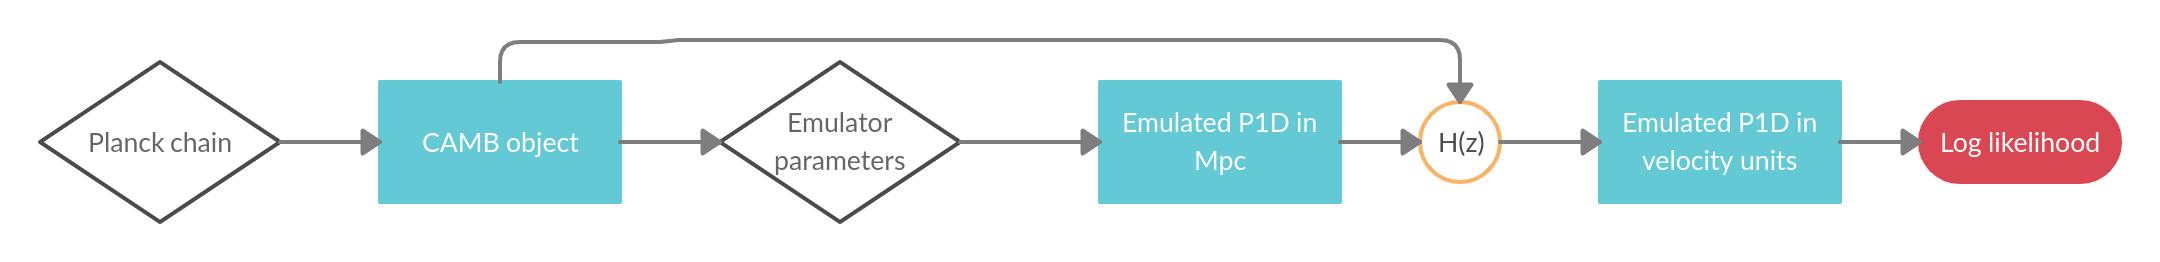
\includegraphics[scale=0.2]{Figures/Parameter_mapping.png}
    \end{center}
    \caption{Procedure for evaluating a \lyaf\ likelihood for a given
    point in the Planck chain using the full emulator. For each cosmological
    model, a \textsc{CAMB} object is created, and the emulator parameters defined
    in equations \ref{eq:Delta2_p} and \ref{eq:n_p} are calculated. The $H(z)$ calculated
    for each model is then used to convert the comoving emulated \fluxpower\
    to velocity units, and a log likelihood is calculated.}
    \label{fig:param_map1}
\end{figure}

In Fig \ref{fig:param_map2}, we show an alternative approach, where the compressed
parameters are calculated for each point in the Planck chain, which are then used
to make the emulator calls, and a fiducial $H(z)$ is used for the conversion to
velocity units. If we can show that the effect on the posteriors of adding the \lyaf\
contributions to the likelihoods is the same whether we follow either of these
approaches, we believe that this demonstrates that all of the necessary information
is contained within the compressed parameters.

\begin{figure}[ht]
    \begin{center}
     
\includegraphics[scale=0.2]{Figures/Compressed_test.png}
    \end{center}
    \caption{Here we evaluate each \lyaf\ likelihood contribution going
    through the compressed likelihood parameters. Intsead of calculating
    the emulator calls directly from the cosmological model, the compressed
    likelihood parameters are calculated first, and these are then used to
    find the emulator parameters. A fiducial expansion rate is then used for
    the conversion of the emulated \fluxpower\ to velocity units.}
    \label{fig:param_map2}
\end{figure}

Once we have demonstrated this, studies of the \lyaf\ could be combined with other
probes using the approach in Fig \ref{fig:param_map3}. The expert users of the emulator
will calculate marginalised posteriors for the compressed likelihood parameters which
can be included in packages such as \textsc{CosmoMC} and \textsc{MontePython}, from
which point onwards it becomes trivial to combine the \lyaf\ with other probes.

\begin{figure}[ht]
    \begin{center}
     
\includegraphics[scale=0.2]{Figures/Marginalised_compressed.png}
    \end{center}
    \caption{Once we have demonstrated that there is no significant loss of
    information when using the compressed likelihood parameters, \lyaf\ results
    could be combined with other probes using this procedure.}
    \label{fig:param_map3}
\end{figure}

\subsection{Adding flexibility to the growth rate and expansion history}
\label{ss:extensions}
In the previous approach we have kept fixed the expansion history and growth rate.
There is a physical motivation for doing so, as these quantities are close to
independent of cosmological model. However whether these approximations are appropriate
for the most recent and future observations is an open question. In order to test this,
we introduce to the compressed likelihood parameter space two parameters, which allow for
some variation in the growth rate and expansion history respectively.

\begin{equation}
    f(z) = \frac{\partial \ln D(z)}{\partial \ln a(z)}
     = - \frac{\partial \ln D(z)}{\partial \ln (1+z)}
     = - \frac{1}{2} \frac{\partial \ln P(z,k)}{\partial \ln (1+z)} ~,
\end{equation}

\begin{equation}
    g_\ast = \frac{2}{3} \frac{1+z_\ast}{H_\ast} 
         \frac{\partial H(z)}{\partial z} \Bigr\rvert_{z_\ast} ~.
\end{equation}

To what extent we are sensitive to these parameters, and the effect that opening
up some variation in them will have on our constraints on the linear power is
something I am currently working on, and it is not year clear whether we will
want to include them in the final set of marginalised compressed likelihood
parameters.

\CP{I'm tempted to leave definitions of these quantities out entirely.
Defining them properly will require a fair bit of volume and could end
up being distracting. Shall we leave a thorough definition of these
quantities to a future document? I'm aware what I have right now
isn't coherent and self contained}

\bibliography{main}
\bibliographystyle{JHEP}

\end{document}
